%!TEX program = xelatex

\documentclass[usepdftitle=false]{beamer}

% Good bibliography
\RequirePackage[backend=biber]{biblatex}
\addbibresource[datatype=bibtex]{biblio.bib}

\RequirePackage{hyperref}

\hypersetup{
	pdftitle			= {Sarek, a portable workflow for WGS analysis of germline and somatic mutations},
	pdfsubject		= {Presentation at JOBIM 2018},
	pdfkeywords		= {Somatic, Germline, Variations, Cancer, Workflow, Container, Reproducibility, Nextflow, Pipeline, Singularity, Docker, Genomics},
	pdfauthor			= {Maxime U. Garcia},
	pdfcreator		= {\LaTeX},
	pdfproducer		= {XeTeX 3.14159265-2.6-0.99996}}

% Icon Fonts
\RequirePackage{academicons}
\RequirePackage{fontawesome}

% Correct the path when including svg pictures
\RequirePackage{import}

% For nice verbatim
\RequirePackage{minted}
\definecolor{LightGray}{HTML}{D3D3D3}
\setmintedinline{bgcolor=LightGray}

% To resize graphic and table
\RequirePackage{graphics}

% For captions
\RequirePackage{caption}

% Arrange theme
\usetheme[
	progressbar=frametitle,
	sectionpage=none,
	numbering=fraction
]{metropolis}

\makeatletter
	\setlength{\metropolis@titleseparator@linewidth}{1pt}
	\setlength{\metropolis@progressonsectionpage@linewidth}{2pt}
	\setlength{\metropolis@progressinheadfoot@linewidth}{2pt}
\makeatother

% Color the progress:
% - SciLifeLabGreen (#7FCB28) for SciLifeLab
% - violet for KI
\definecolor{SciLifeLabGreen}{HTML}{7FCB28}
\setbeamercolor{progress bar}{fg=SciLifeLabGreen,bg=white}

\newcommand{\ts}{\textsuperscript}

\title{%
	\vspace{-.8cm}%
	Sarek
}

\subtitle{%
	\normalsize{A portable workflow for WGS analysis\\of germline and somatic mutations}%
	\vspace{-.4cm}%
}

\titlegraphic{
	\hfill
\includegraphics[height=.8cm]{pictures/SciLifeLab-white}%
	\vspace{.3cm}%

	\hfill
\includegraphics[height=.8cm]{pictures/NGI-white}%
	\vspace{.5cm}%

	\hspace{7.7cm}
\includegraphics[height=1.2cm]{pictures/KI-white}%
	\hfill\includegraphics[height=1.2cm]{pictures/Barntumörbanken-logo}%
}

\author{
	\vspace{-.6cm}
	\faUser\ Maxime U. Garcia\\
	\faGlobe\ \href{https://maxulysse.github.io/}{maxulysse.github.io}\\
	\faGithub\ \href{https://github.com/MaxUlysse/}{@MaxUlysse}\\
	\faTwitter\ \href{https://twitter.com/gau/}{@gau}\\
	\\
	
\includegraphics[height=.7cm]{pictures/JOBIM2018-white}
}

\date{\vfill}

\begin{document}

\section{Sarek}

{
	\usebackgroundtemplate{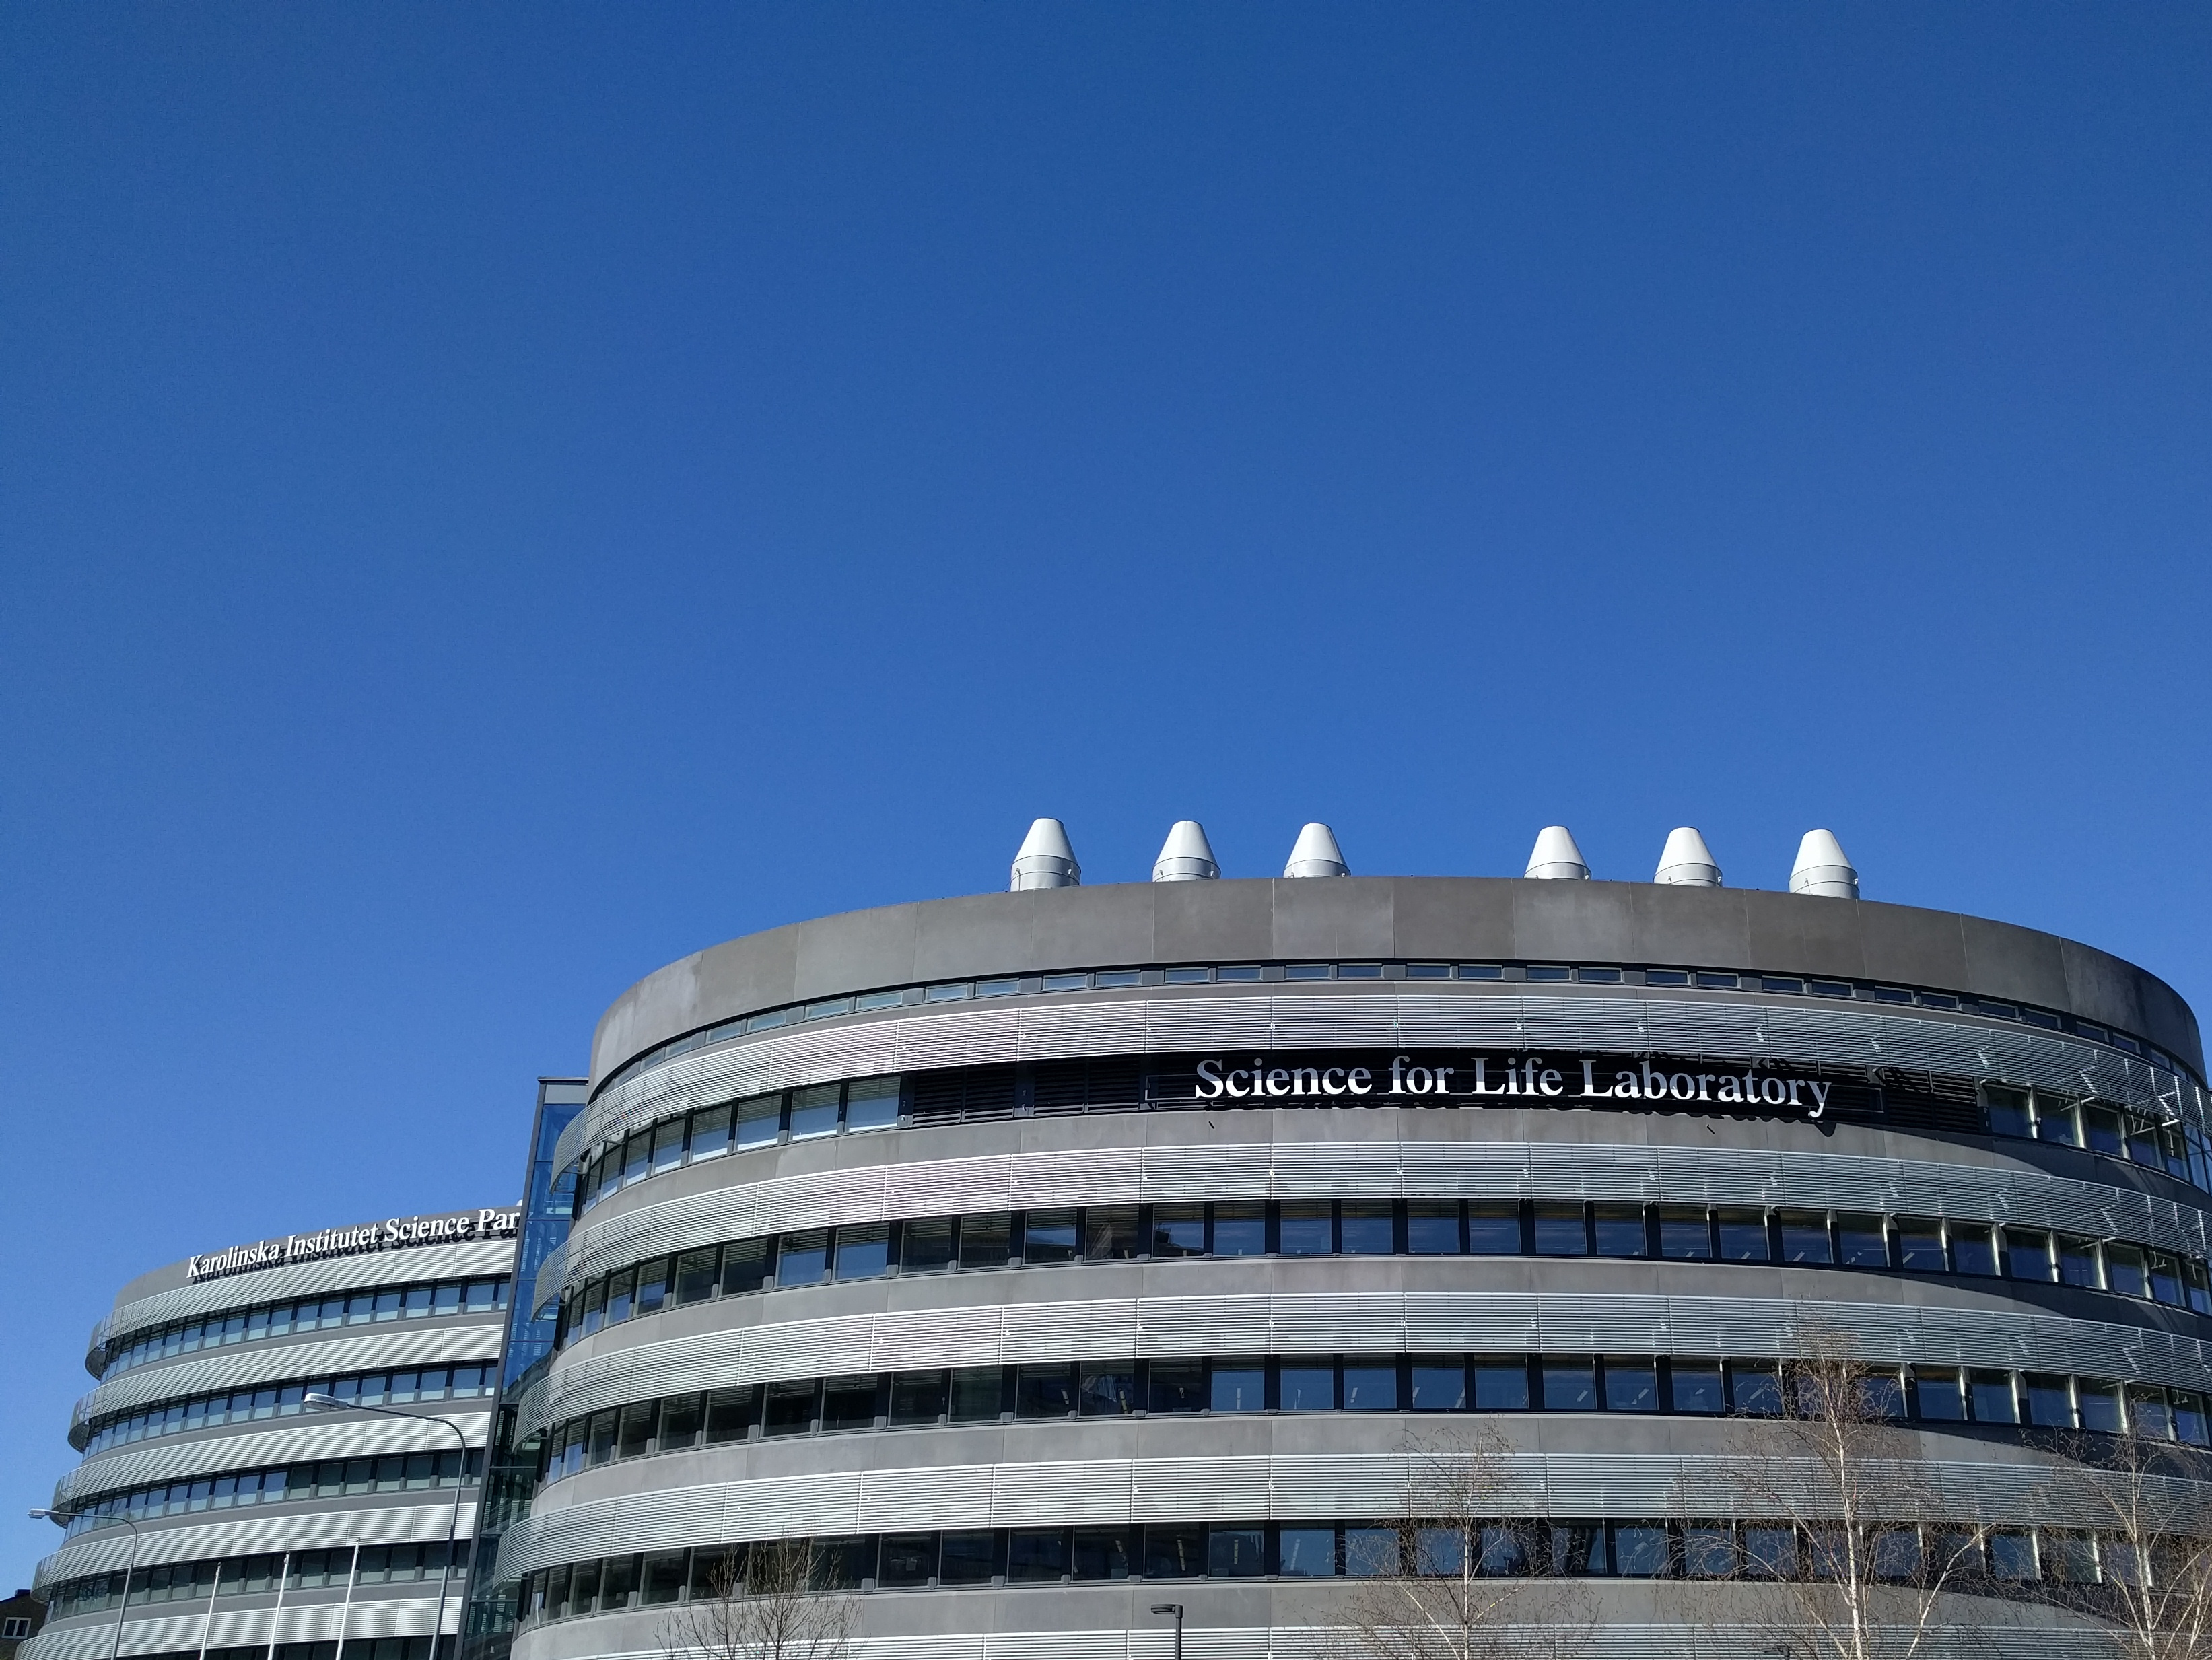
\includegraphics[width=\paperwidth]{pictures/SciLifelab-BlueSky2.jpg}}
	\setbeamercolor{normal text}{fg = white, bg = white}
	\maketitle
}

\section{Science for Life Laboratory}

\begin{frame}{Science for Life Laboratory}
	\begin{figure}
		
\includegraphics[height=1.5cm]{pictures/SciLifeLab}
		\captionof*{figure}{\faGlobe\ \url{https://scilifelab.se/}}
	\end{figure}
	\only<1>{
		\centering SciLifeLab is a national centre for molecular biosciences\\with focus on health and environmental research

		\begin{figure}
			\hfill%
			
\includegraphics[height=1.58cm]{pictures/KI}%
			\hfill%
			
\includegraphics[height=1.58cm]{pictures/KTH}%
			\hfill%
			
\includegraphics[height=1.58cm]{pictures/SU}%
			\hfill%
			
\includegraphics[height=1.58cm]{pictures/UU}%
			\hfill%
			\hfill%
		\end{figure}
	}
	\only<2>{
		\centering Infrastructure Services

		\begin{table}
			\resizebox{.8\textwidth}{!}{%
			\begin{tabular}{lll}
				Genomics 						&	Proteomics								&	Metabolomics \\
														&														& \\
				Single Cell Biology	&	Bioimaging and Molecular	&	Chemical Biology and Genome \\
														&	 Structure								&	Engineering \\
														&														& \\
				Drug Discovery 			&	Diagnostics								&	Bioinformatics \\
			\end{tabular}}
		\end{table}
	}
\end{frame}

\begin{frame}{National Genomics Infrastructure}
	\begin{figure}
		
\includegraphics[height=.7cm]{pictures/NGI}
		\captionof*{figure}{\faGlobe\ \url{https://ngisweden.scilifelab.se/}}
	\end{figure}

	
\includegraphics[height=.8cm]{pictures/blank}
	\begin{itemize}
		\item National resource
		\pause
		\item State-of-the-art infrastructure
		\begin{itemize}
			\item massively parallel DNA sequencing and SNP genotyping
		\end{itemize}
		\pause
		\item Guidelines and support
		\begin{itemize}
			\item sample collection, study design, protocol selection
			\item bioinformatics analysis
			\end{itemize}
	\end{itemize}
	
\includegraphics[height=.8cm]{pictures/blank}

\end{frame}

\begin{frame}{National Bioinformatics Infrastructure Sweden}
	\begin{figure}
		
\includegraphics[height=.7cm]{pictures/NBIS}
		\captionof*{figure}{\faGlobe\ \url{https://www.nbis.se/}}
	\end{figure}

	\only<1-2>{
		
\includegraphics[height=2cm]{pictures/blank}
		\begin{itemize}
			\item Swedish ELIXIR node
			\pause
			\item Bioinformatics support for Swedish researchers
		\end{itemize}
		
\includegraphics[height=2cm]{pictures/blank}
	}

	\only<3>{
		\begin{figure}
			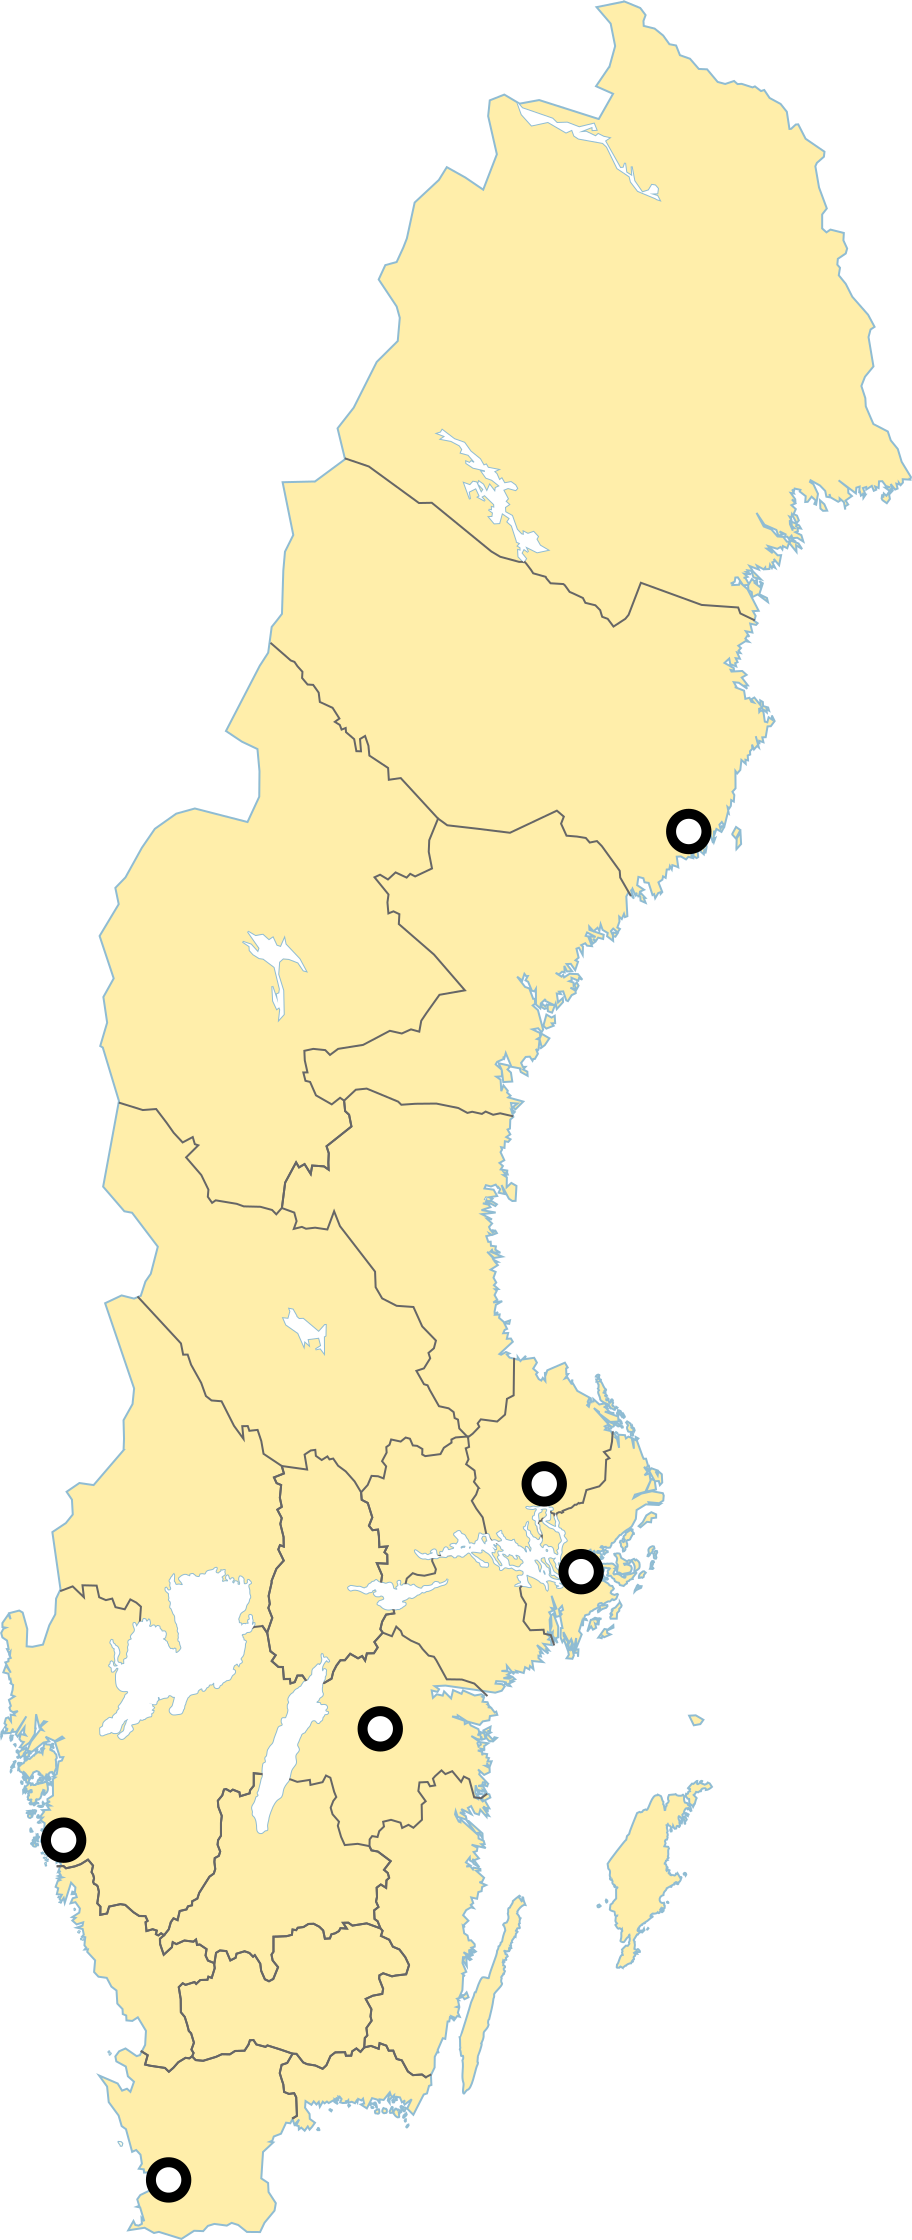
\includegraphics[height=5cm]{pictures/Sweden-map-NBIS.png}
		\end{figure}
	}

\end{frame}

\section{Sarek}

\begin{frame}{Sarek}
	\only<1>{
		\begin{figure}
			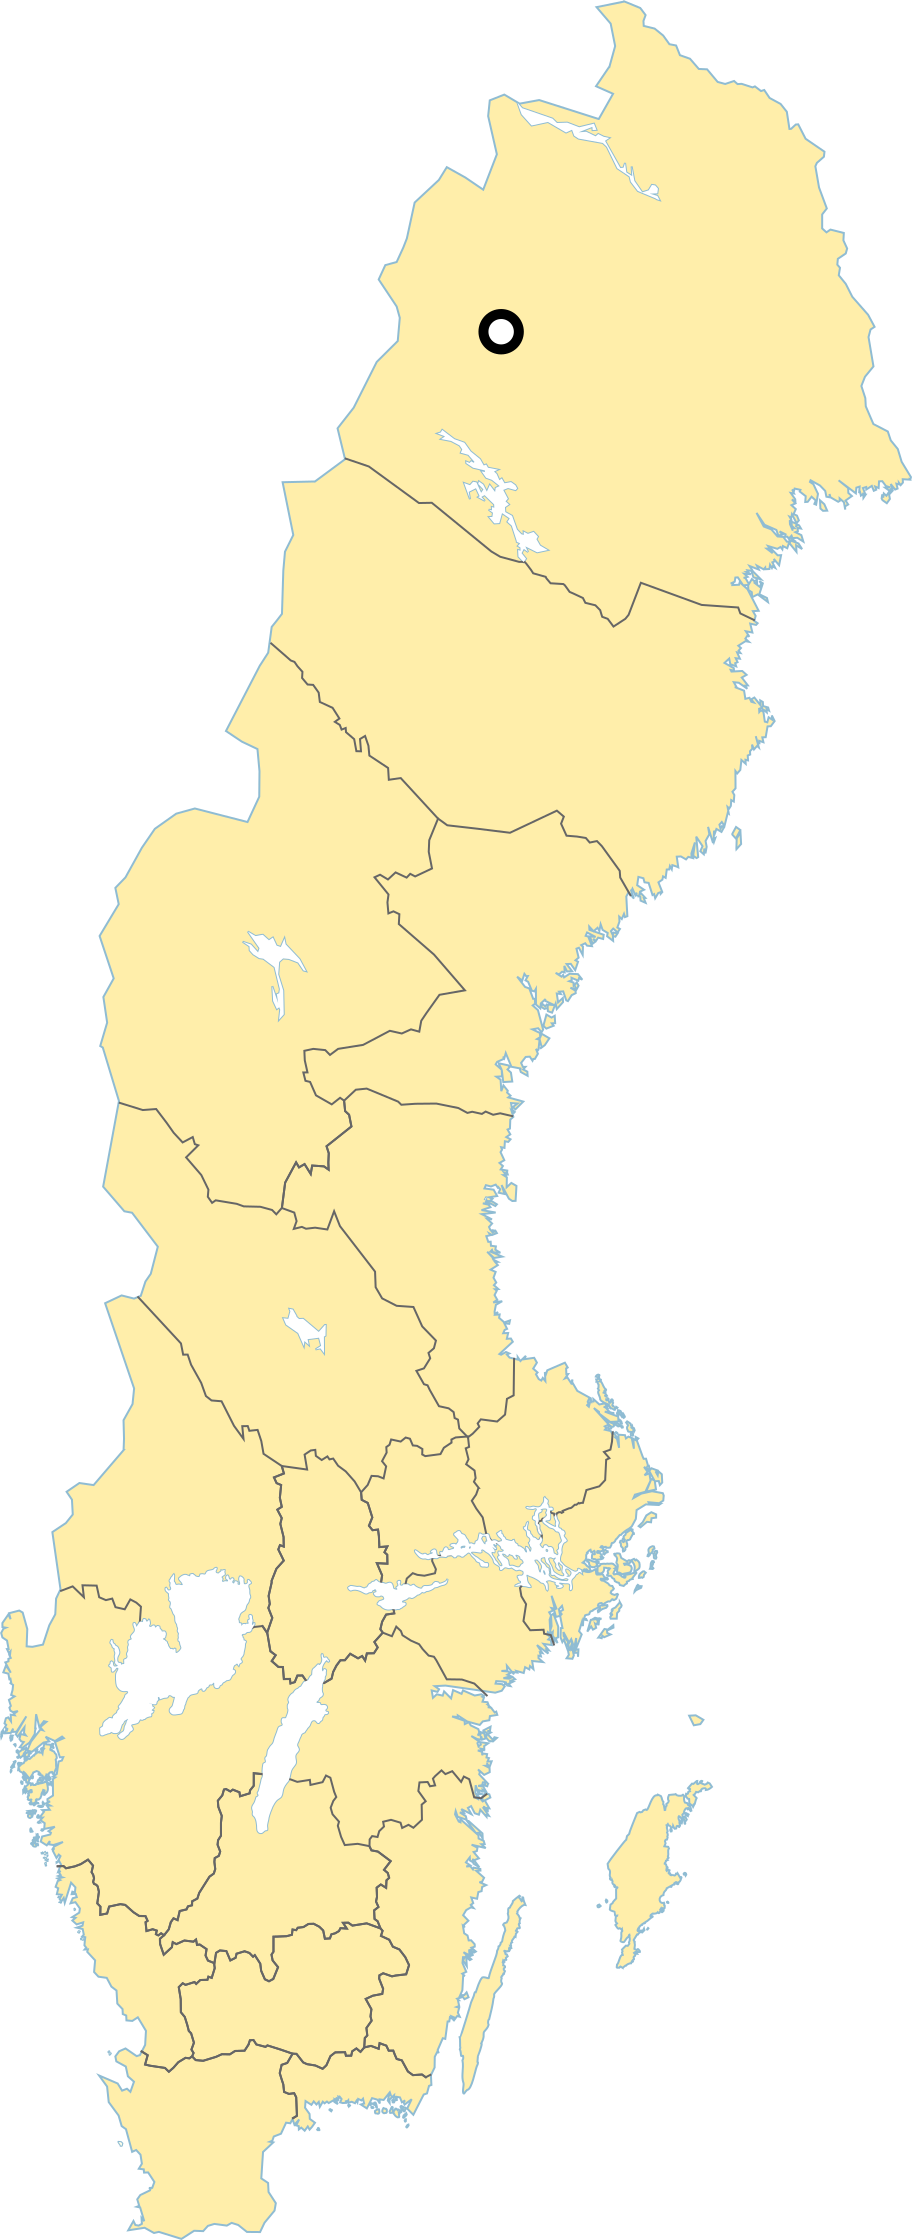
\includegraphics[height=8cm]{pictures/Sweden-map-Sarek.png}
		\end{figure}
	}
	\only<2>{
		\begin{figure}
			\includegraphics[height=7cm]{pictures/Skierfe-summer.jpg}
			\captionof*{figure}{Sarek, the National Park in Northen Sweden}
		\end{figure}
	}
\end{frame}

\begin{frame}{The most dramatic and grandiose of all}
	\begin{itemize}
		\item Long, deep, narrow valleys and wild, turbulent water.
		\item \textbf{A tortuous delta landscape.}
		\item Completely lacking in comfortable accommodations.
		\item Sarek is one of Sweden’s \textbf{most inaccessible national parks}
		\item \textbf{There are no roads leading up to the national park}.
	\end{itemize}
	\hfill\href{http://www.nationalparksofsweden.se/choose-park---list/sarek-national-park/national-park-fact/}{Sarek National Park website}
\end{frame}

\begin{frame}{Where we're going we don't need roads}
	\begin{figure}
		
\includegraphics[height=6.5cm]{pictures/OneDoesNotSimply-meme.png}
	\end{figure}
\end{frame}

\begin{frame}{What is Sarek?}
	\begin{figure}
		
\includegraphics[height=1cm]{pictures/Sarek_no_border}
		\captionof*{figure}{\faGlobe\ \url{http://opensource.scilifelab.se/projects/sarek/}}
	\end{figure}
	\begin{itemize}
		\pause
		\item Nextflow pipeline
		\item<3-> Developed at NGI
		\item<4-> In collaboration with NBIS
		\item<5-> Support from The Swedish Childhood Tumor Biobank
	\end{itemize}
	\begin{figure}
		
\includegraphics[height=1cm]{pictures/blank}<-2>
		
\includegraphics[height=1cm]{pictures/NGI}<3->
		\only<3->{\hfill}
		\includegraphics[height=1cm]{pictures/Barntumörbanken-logo}<5->
		\only<4->{\hfill}
		
\includegraphics[height=1cm]{pictures/NBIS}<4->
	\end{figure}
	\vfill
\end{frame}

\section{Under the hood}

\begin{frame}{Nextflow}
	\begin{figure}
		
\includegraphics[height=1cm]{pictures/nextflow.png}
		\captionof*{figure}{\faGlobe\ \url{https://www.nextflow.io/}}
		
\includegraphics[height=1cm]{pictures/blank}
	\end{figure}
	\begin{itemize}
		\item Data-driven workflow language
		\pause
		\item Portable (executable on multiple platforms)
		\pause
		\item Shareable and reproducible (with containers)
	\end{itemize}
	\vfill
\end{frame}

\begin{frame}{Singularity}
	\begin{figure}
		
\includegraphics[height=1cm]{pictures/Singularity}
		\captionof*{figure}{\faGlobe\ \url{https://singularity.lbl.gov/}}
		
\includegraphics[height=1cm]{pictures/blank}
	\end{figure}
	\begin{itemize}
		\item Docker-like container engine
		\item Specific for HPC environnment
		\pause
		\item Without the root user security problem
		\pause
		\item Supported by Nextflow
		\pause
		\item Can pull containers from Docker-hub
	\end{itemize}
\end{frame}

\section{What's inside}

\begin{frame}{Sarek exists in two flavors}
	\begin{figure}
		
\includegraphics[height=1.5cm]{pictures/Sarek}
	\end{figure}
	\vfill
	\pause
	\begin{center}
		
\includegraphics[height=1.5cm]{pictures/Sarek_germline}
		\hfill
		\pause
		
\includegraphics[height=1.5cm]{pictures/Sarek_somatic}
	\end{center}
	\end{frame}

\begin{frame}{Preprocessing}
	\begin{figure}
		
\includegraphics[height=1cm]{pictures/GATKBP}
		\captionof*{figure}{\faGlobe\ \url{https://software.broadinstitute.org/gatk/best-practices/}}
	\end{figure}
	Based on GATK Best Practices (GATK 3.8)

	\faWrench\ Switching to GATK 4.0
	\pause

	\begin{itemize}
		\item Reads mapped to reference genome with \mintinline{text}{bwa}
		\pause
		\item Duplicates marked with \mintinline{text}{picard MarkDuplicates}
		\pause
		\item Realign indels with \mintinline{text}{GATK IndelRealigner}
		\pause
		\item Recalibrate with \mintinline{text}{GATK BaseRecalibrator}
	\end{itemize}

\end{frame}

\begin{frame}{Germline Variant Calling}
	\begin{itemize}
		\item SNVs and small indels:
		\pause
	\begin{itemize}
			\item HaplotypeCaller
			\item Strelka2
		\end{itemize}
		\pause
		\item Structural variants:
		\pause
		\begin{itemize}
			\item Manta
		\end{itemize}
	\end{itemize}
\end{frame}

\begin{frame}{Somatic Variant Calling}
	\begin{itemize}
		\item SNVs and small indels:
		\pause
		\begin{itemize}
			\item MuTect1 (\faWrench\ removing)
			\item MuTect2
			\item Freebayes
			\item Strelka2
		\end{itemize}
		\pause
		\item Structural variants:
		\pause
		\begin{itemize}
			\item Manta
		\end{itemize}
		\pause
		\item Sample heterogeneity, ploidy and CNVs:
		\pause
		\begin{itemize}
			\item ASCAT
			\item Control-FREEC (\faWrench\ adding)
		\end{itemize}
	\end{itemize}
\end{frame}

\begin{frame}{SNV Calling overlap}
	\begin{figure}
		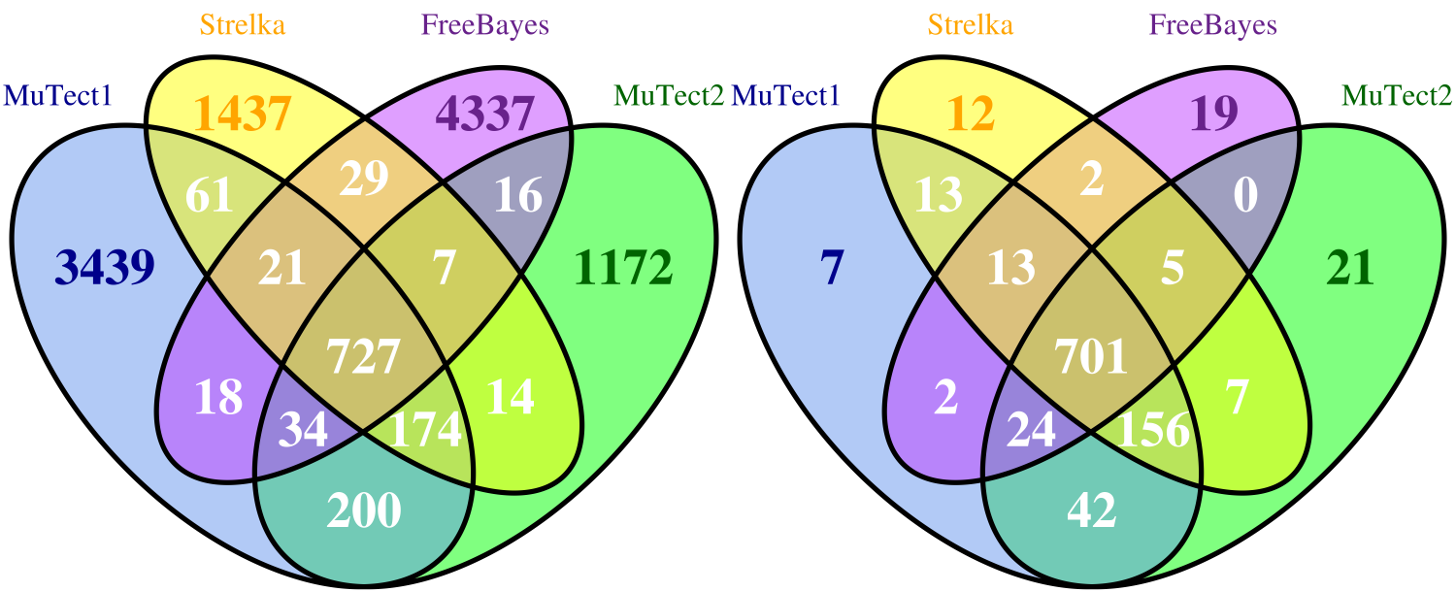
\includegraphics[height=4cm]{pictures/Sarek_venn_Calls.png}
	\end{figure}
		\vspace{-.5cm}
		\begin{center}
			\small{All calls\hspace{2cm}\ True positives only}
		\end{center}

		\small{Number and overlap of somatic SNV calls from a WGS medulloblastoma dataset}

	\small{Alioto TS et al. (2015) \aiDoi\ \url{https://doi.org/10.1038/ncomms10001}}
\end{frame}

\begin{frame}{Annotation}
	\begin{itemize}
		\item VEP and SnpEff
		\pause
		\item \faDatabase\ ClinVar, COSMIC, dbSNP, GENCODE, gnomAD, polyphen, sift, etc.
	\end{itemize}
\end{frame}

\begin{frame}{\faWrench\ Prioritization}
	\begin{itemize}
		\item	First step towards clinical use
		\pause
		\item	Rank scores are computed for all variants
		\begin{itemize}
			\item	COSMIC, ClinVar, SweFreq and MSK-IMPACT (cancerhotspots.org)
		\end{itemize}
		\pause
		\item	Findings are ranked in three tiers
		\pause
		\begin{itemize}
			\item	1\ts{st} tier: well known, high-impact variants
			\item	2\ts{nd} tier: variants in known cancer-related genes
			\item	3\ts{rd} tier: the remaining variants
		\end{itemize}
	\end{itemize}
\end{frame}

\begin{frame}{Reports}
	\begin{figure}
		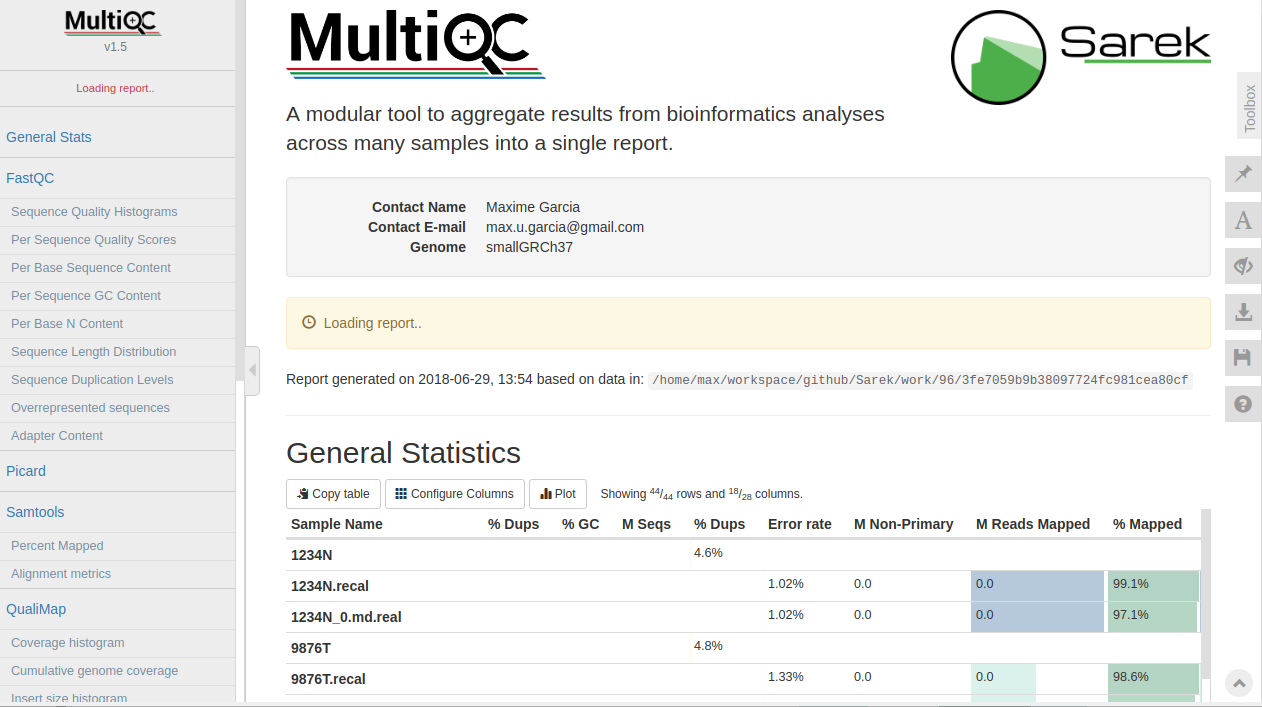
\includegraphics[height=6cm]{pictures/MultiQC_screenshot-2018-07-02.png}
		\captionof*{figure}{\faGlobe\ \url{http://multiqc.info/}}
	\end{figure}
\end{frame}

\begin{frame}{Workflow}
	\begin{figure}
		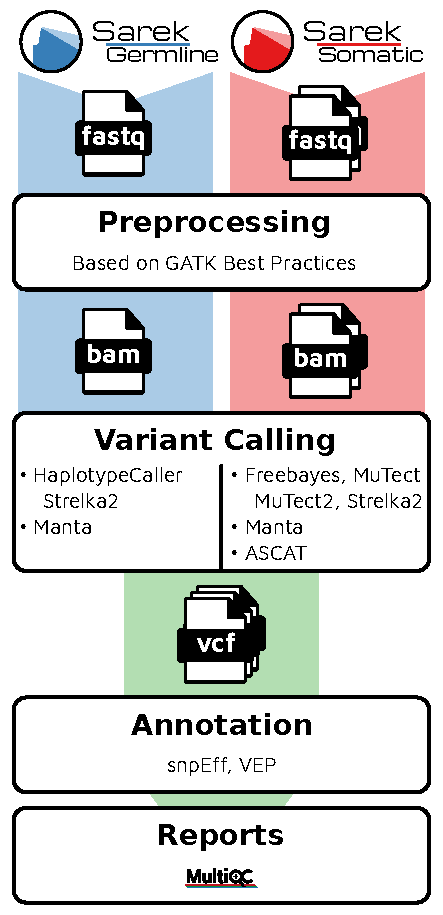
\includegraphics[height=7cm]{pictures/Sarek_workflow_2}
	\end{figure}
\end{frame}

\section{What's next}

\begin{frame}{WES and gene panels}
	\begin{itemize}
		\item Preprocessing is done with the whole genome
		\pause
		\item Variant call only on the target regions
	\end{itemize}
\end{frame}

\begin{frame}{Reference genomes}
	\begin{itemize}
		\item GRCh37 and GRCh38
		\pause
		\item Custom genome
	\end{itemize}
\end{frame}

\begin{frame}{Sarek at work}
	\begin{itemize}
		\item	50 tumor/normal pairs with GRCh37 reference
		\pause
		\item	90 tumor/normal pairs (with some relapse) with GRCh38 reference
		\pause
		\item	The whole SweGen dataset with GRCh38 reference
		\begin{itemize}
			\item	1 000 samples in germline settings
		\end{itemize}
		\pause
		\item	4 clinical samples
		\begin{itemize}
			\item	more coming with Genomic Medicine Sweden initiative
		\end{itemize}
	\end{itemize}
\end{frame}

\begin{frame}{\faWrench\ Preprint available at BioRxiv}

	\textbf{Sarek: A portable workflow for whole-genome sequencing analysis of germline and somatic variants}

	\small{Maxime Garcia,
	Szilveszter Juhos,
	Malin Larsson,
	Pall I Olason,
	Marcel Martin,
	Jesper Eisfeldt,
	Sebastian DiLorenzo,
	Johanna Sandgren,
	Teresita Diaz de Ståhl,
	Valtteri Wirta,
	Monica Nistèr,
	Björn Nystedt,
	Max Käller}

	\aiDoi\ \url{https://doi.org/10.1101/316976}
\end{frame}

\section{nf-core}

\begin{frame}{nf-core}
	\begin{figure}
		
\includegraphics[height=1cm]{pictures/nf-core}
		\captionof*{figure}{\faGlobe\ \url{http://nf-co.re/}}
	\end{figure}
	A community effort to collect a curated set of Nextflow analysis pipelines
	\begin{itemize}
		\item GitHub organisation to collect pipelines in one place
		\item No institute-specific branding
		\item Strict set of guideline requirements
		\item Automated testing for code style and function
		\item Conda environnment, Docker and Singularity container
	\end{itemize}
\end{frame}

\section{Acknowledgments}

\begin{frame}{Get involved!}
	\begin{itemize}
		\item Our code is hosted on Github

		\faGithub\ \url{https://github.com/SciLifeLab/Sarek}

		\faGithub\ \url{https://github.com/nf-core}
	\end{itemize}
	\pause
	\begin{itemize}
		\item We have gitter channels

		\faGroup\ \url{https://gitter.im/SciLifeLab/Sarek}

		\faGroup\ \url{https://gitter.im/nf-core/Lobby}
	\end{itemize}
\end{frame}

\begin{frame}{Acknowledgments}
	\begin{figure}
		
\includegraphics[height=.6cm]{pictures/Barncancerfonden}%
		\hfill%
		
\includegraphics[height=.6cm]{pictures/KI}%
		\hfill%
		\includegraphics[height=.6cm]{pictures/Barntumörbanken-logo}%
		\hfill%
		
\includegraphics[height=.6cm]{pictures/SciLifeLab}%
		\hfill%
		
\includegraphics[height=.6cm]{pictures/uppmax.png}%
	\end{figure}
	\begin{table}
		\resizebox{.7\textwidth}{!}{%
		\begin{tabular}{lll}
		\textbf{Barntumörbanken}		&	\textbf{NGI}								&	\textbf{NBIS}							\\
		Elisa Basmaci								&	Anandashankar Anil					&	Sebastian DiLorenzo				\\
		Szilveszter Juhos						&	Orlando Contreras‐López			&	Malin Larsson							\\
		Gustaf Ljungman							&	Phil Ewels									&	Marcel Martin							\\
		Monica Nistèr								&	Sofia Haglund								&	Markus Mayrhofer					\\
		Gabriela Prochazka					&	Max Käller									&	Björn Nystedt							\\
		Johanna Sandgren						&	Anna Konrad									&	Markus Ringnér						\\
		Teresita Díaz De Ståhl			&	Pär Lundin									&	Pall I Olason							\\
		Katarzyna Zielinska-Chomej	&	Remi-Andre Olsen						&	Jonas Söderberg						\\
																&	Senthilkumar Panneerselvam	&														\\
		\textbf{Grupp Nistèr}				&	Fanny Taborsak							&	\textbf{Clinical Genomics}\\
		Saad Alqahtani							&	Chuan Wang									&	Kenny Billiau							\\
		Min Guo											&															&	Hassan Foroughi Asl				\\
		Daniel Hägerstrand					&	\textbf{Nextflow folks}			&	Valtteri Wirta						\\
		Anna Hedrén									&	Paolo Di Tommaso						&														\\
		Rong Yu											&	Alexander Peltzer						&	\textbf{Clinical Genetics}\\
		Jian Zhao										&	Sven Fillinger							&	Jesper Eisfeldt						\\
		\end{tabular}}
	\end{table}
	\begin{figure}
		
\includegraphics[height=.6cm]{pictures/NGI}%
		\hfill%
		
\includegraphics[height=.6cm]{pictures/NBIS}%
		\hfill%
		
\includegraphics[height=.6cm]{pictures/nextflow.png}%
		\hfill%
		
\includegraphics[height=.6cm]{pictures/nf-core}%
	\end{figure}
\end{frame}

{
	\usebackgroundtemplate{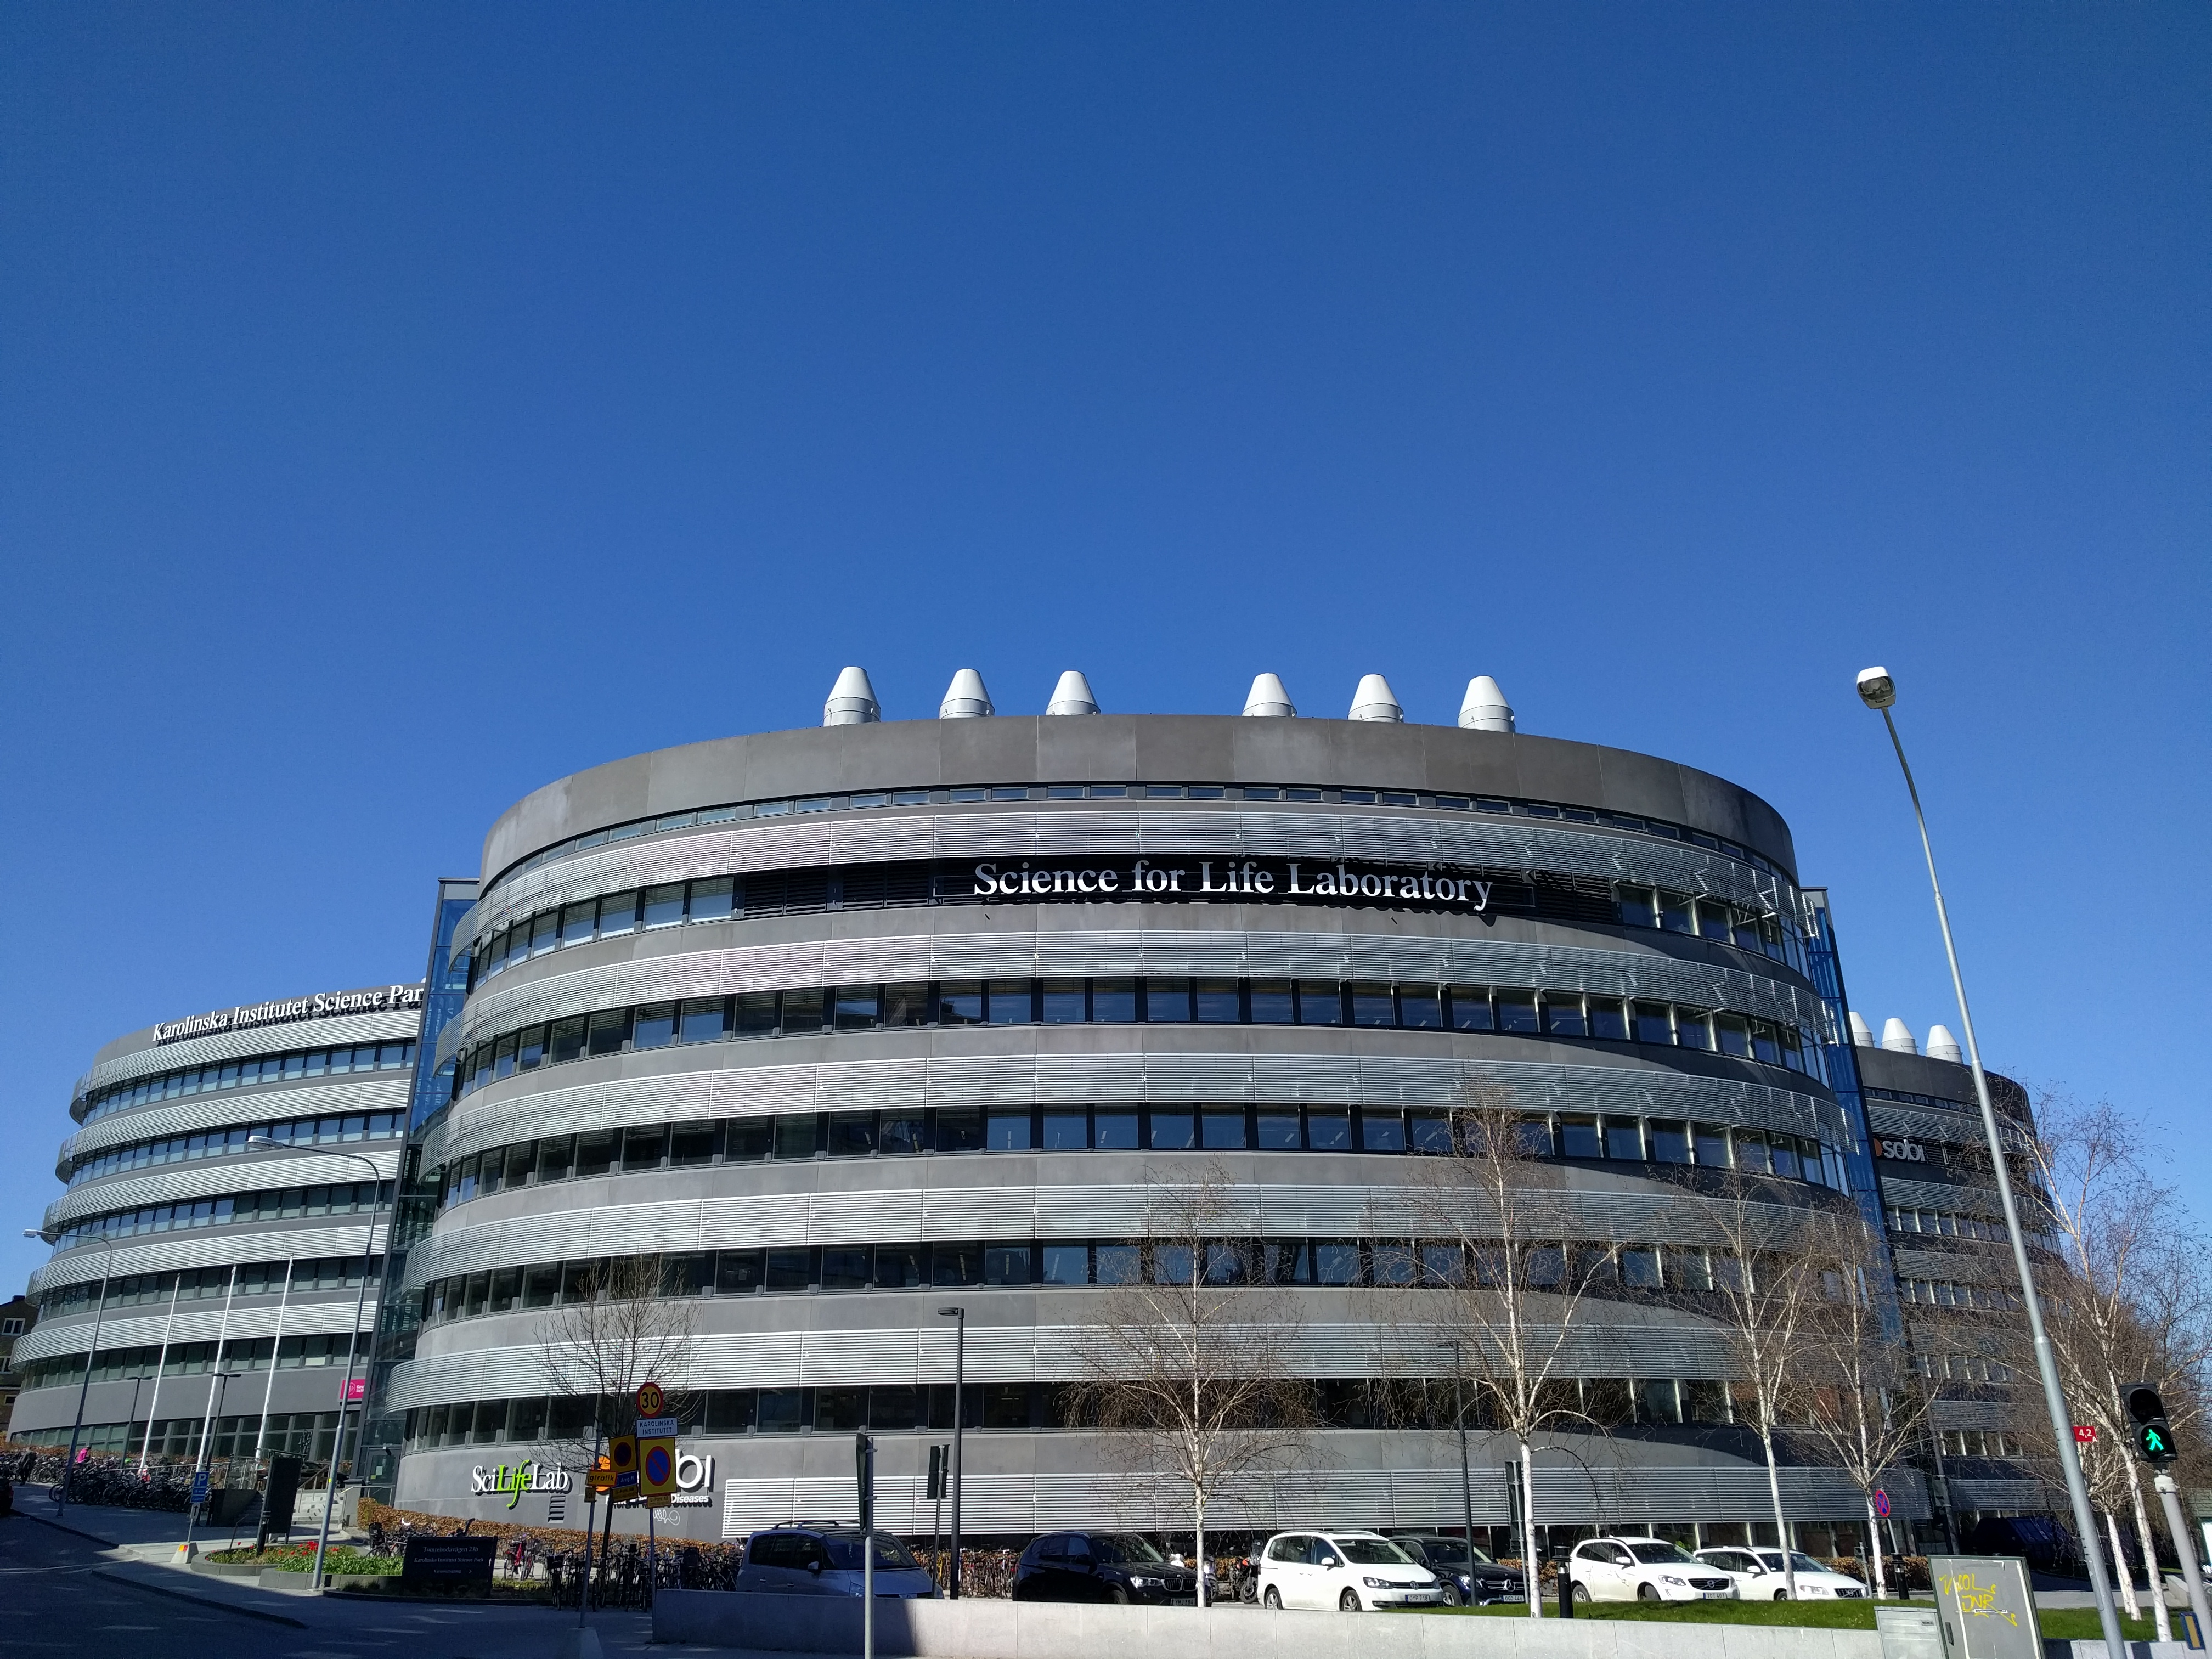
\includegraphics[width=\paperwidth]{pictures/SciLifelab-BlueSky.jpg}}
	\setbeamercolor{normal text}{fg = white}
	\setbeamercolor{frametitle}{fg = white, bg = black!80}
	\usebeamercolor[fg]{normal text}
	\section{Questions}
	\begin{frame}[plain]{Any questions?}
	\vspace{-6cm}
	\faGlobe\ \url{http://opensource.scilifelab.se/projects/sarek/}

	\faGithub\ \url{https://github.com/SciLifeLab/Sarek}

	\faGlobe\ \url{https://maxulysse.github.io/jobim2018}
	\end{frame}
}

\end{document}
